\documentclass[11pt]{article}

\usepackage[french, english]{babel}

\usepackage[T1]{fontenc}

\usepackage{amsfonts}
\usepackage{amsmath}
\usepackage{amssymb}

\usepackage{graphicx}
\usepackage{multirow}
\usepackage{multicol}
\usepackage{xcolor}
\usepackage[shortlabels]{enumitem}

\usepackage[margin=2cm]{geometry}

\usepackage{mathtools}
\usepackage{siunitx}
\usepackage{braket}

\usepackage{listings}
\renewcommand\lstlistingname{Code Python}

\lstset{frame=tb,
  language=Python,
  numbers=left,
  stepnumber=1,
  aboveskip=3mm,
  belowskip=3mm,
  showstringspaces=false,
  columns=flexible,
  basicstyle={\small\ttfamily},
%   numbers=none,
  numberstyle=\tiny\color{gray},
  keywordstyle=\color{blue},
  commentstyle=\color{paired2b},
  stringstyle=\color{paired3b},
  breaklines=true,
  breakatwhitespace=true,
  tabsize=1,
  frame=single,
%   showtabs=false,
}


\begin{document}


\hrule

\begin{center}
  {\Large GEI299 - Gestion de projet} \\ \vspace{5mm}
  {\LARGE\sffamily Devoir 1} \\
  Alexis Jean \\
  À remettre le 25 septembre
\end{center}

\hrule


\section{\underline{Introduction au contract}}
Le client M. Scanner de la compagnie GE Healthcare souhaite explorer les possibilités de différents métaux pouvant être utilisés comme agent de contraste dans les images de résonance magnétique (IRM). La raison, l'agent de contraste en utilisation actuelle, le gadolinium, est trop toxique pour le client. Ce dernier requiert de notre expertise pour développer un logiciel pouvant sélectionner un candiat de remplaçement parmis différents critères qui seront mentionnés plus loin de le document.


\section{\underline{Éléments à inclure, contraintes et points à clarifier}}

\subsection{Éléments à inclure}
Dans la section qui suit, les éléments à inclure ainsi que les contraintes du client seront présentés sous forme de deux listes de puces. Selon les demandes du client, il nous faudra apporter les suivantes fonctionnalités comme nécessité au produit qui est demandé :

\begin{itemize}[label=\textbullet]
  \item Une interface utilisateur simple et intuitive au couleur de GE Healthcare
  \item Le logiciel doit permettre l'ajout, la modification et la supression de métaux de la base de données jugés comme candidats potentiels
  \item Un module de simulation quantique (via la plateforme de IBM) doit être intégrée pour pouvoir calculer l’état fondamental et les propriétés électroniques des complexes métal-ligand
  \item Une façon de pouvoir comparer les différents candidats selon différents critères
  \item Avoir la possibilité de pouvoir exporter les résultats sous différents formats
  \item Le logiciel doit avoir deux modes : un mode scientifique et un mode affaires
\end{itemize}

\subsection{Contraintes}
Le client a aussi des contraintes qui viennent avec sa demande qui se listent tel que :

\begin{itemize}
  \item Le logiciel doit compatible avec autant Windows que MacOS
  \item Le temps de calcul pour un simulation standard doit être inférieur à 2 minutes et d'avoir un taux d'erreur inférieur à 2\%
  \item Un langage et un framework maintenable avec une connexion sécurisée à la plateforme IBM Quantum pour l’exécution des calculs sont nécessaires
  \item Le budget maximal permis est de 200 000\$ qui couvre le matériel quantique, les ressources humaines ainsi que le matériel
  \item Le produit final doit être livré au bout de 2 mentionnés
  \item Le code doit être modulaire pour des ajouts et doit posséder un plan de maintenance sur 12 mois
\end{itemize}

\subsection{Points à clarifier}
Dans l'analyse de l'énoncé, quelques questions ont été retenues qui doivent être communiquées avec le client pour la bonne continuation du projet. Comme précédemment, les questions seront énoncées sous forme de liste de puces :

\begin{itemize}
  \item Quel est le niveau de détail qui est attendu pour le mode scientifique du logiciel ?
  \item Pour pouvoir comparer les taux d'erreur, comment pouvons-nous obtenir la référence classique ?
  \item Pour ce qui est de l'interface, y'a-t-il une préférence pour le web ou desktop ?
\end{itemize}
Voici un exemple de réponse possible pour chaque question :

\begin{itemize}
  \item Le mode scientifique doit apporter des graphiques, des calculs complets ainsi qu'un rapport complet de chaque simulation
  \item Les références classqieus se trouve dans l'échantillon en pièce jointe dans le matériel du projet
  \item Une terface desktop sera préférée pour aider à la sécurisation des résultats directement sur les machines de la compagnie
\end{itemize}


\section{\underline{Diagramme d'entrées/sorties du logiciel}}
Voici un diagramme des entrées et des sorties du logiciel :

\begin{figure}[h!]
  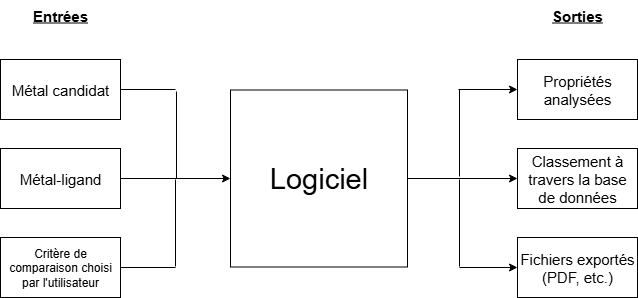
\includegraphics[width=\linewidth]{Diagramme.png}
  \caption{Diagramme entrées/sorties}
\end{figure}

\end{document}







